\scanpage{14}
c)
\[
\begin{aligned}
\unsure{\mathfrak{S}|\mathcal{S}}_4&\simeq\operatorname{Aff}2,\mathbb{F}_2)\simeq\operatorname{GP}(1,\mathbb{F}_3)\\
\unsure{\mathfrak{A}|\mathcal{A}}_4&\simeq\operatorname{Aff}(1,\mathbb{F}_4)\qquad ?
\end{aligned}
\]

d)
\[
\begin{aligned}
\mathfrak{S}_5&\simeq\operatorname{GP}(1,\mathbb{F}_5)\\
\mathfrak{A}_5&\simeq\operatorname{GP}(1,\mathbb{F}_4)
\end{aligned}
\]

Quelques groupes classiques sur un corps $k$

\diagram{\(\left.
\begin{tikzcd}[ampersand replacement=\&,column sep=small,row sep=1em]
1\arrow[r] \& k^*\arrow[r] \& \operatorname{Gl}(V)\arrow[r] \&\operatorname{GP}(V)\arrow[r,dash]\&1\\
1\arrow[r] \& k^*\arrow[r,dash] \&\operatorname{Gl}(n,k)\arrow[r] \&\operatorname{GP}(n-1,k)\arrow[r]\&1
\end{tikzcd}
\right\}\;\text{ne \unsure{splitte} pas en général}\)}

% slanted, in the left margin; the surrounding line has small gaps at the left.
\reversemarginpar
\margin{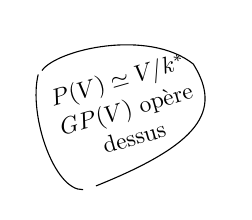
\begin{tikzpicture}[baseline=(proj.base),rotate=16,scale=.85]
\node[inner sep=2pt,transform shape] (proj) {\shortstack{$\mathbb{P}(V)\simeq V/k^*$\\$\operatorname{GP}(V)$ opère\\dessus}};
\draw (-1.05,.88) .. controls (-.75,1.12) and (.65,1.05) .. (1.15,.35)
  .. controls (1.38,-.45) and (.9,-.83) .. (-.75,-1.0);
\draw (-1.12,.84) .. controls (-1.43,.3) and (-1.37,-.9) .. (-.95,-1.0);
\end{tikzpicture}}
\normalmarginpar

\[
\begin{aligned}
\text{Structure de $k$-vectoriel }\tikz[baseline=(vectbase.base)]{
  \node[inner sep=0pt] (vectbase) {sur ens};
  \node[anchor=south west,inner sep=0pt] at ([xshift=-.3em,yshift=.8em]vectbase.north west) {\inserted{de dim $n$}};
  \draw ([xshift=-.35em,yshift=-.4em]vectbase.west)
    .. controls ([xshift=-.7em,yshift=1.0em]vectbase.west) and ([xshift=.4em,yshift=1.1em]vectbase.north west)
    .. ([xshift=.35em,yshift=1.1em]vectbase.north east)
    .. controls ([xshift=.6em,yshift=1.15em]vectbase.north east) and ([xshift=.6em,yshift=1.35em]vectbase.north east)
    .. ([xshift=.4em,yshift=1.35em]vectbase.north east);
}V
&\longleftrightarrow\ \text{donnée d'\unsure{un|une} \unsure{élémt|élément}}\\
&\qquad\text{de }\operatorname{Isom}_{\text{ens}}(k^n,V)/\operatorname{Gl}(n,k)
\end{aligned}
\]

Structure de $k$-espace affine de dim $n$ sur \deleted{$E$} ens $E$
\[
\begin{aligned}
\longleftrightarrow\ &\text{donnée d'un \unsure{élémt|élément} de}\\
&\operatorname{Isom}_{\text{ens}}(k^n,V)/\unsure{\operatorname{Aff}n,k)|\operatorname{Aff}(n,k)}
\end{aligned}
\]

[ De façon \unsure{générale|général}, \deleted{si $Z$ est un \unsure{groupe|grpe}}, la notion de
\tikz[baseline=(oldaff.base)]{
  \node[inner sep=0pt] (oldaff) {\deleted{espace \unsure{affine|aff.}}};
  \node[anchor=south west,inner sep=0pt] at ([xshift=.8em,yshift=.7em]oldaff.north west)
    {\inserted{torseur (à droite, disons) $E$}};
}
sous groupe non précisé peut être considéré comme structure sur le seul ens de base $E$,
\tikz[baseline=(oldapp.base)]{
  \node[inner sep=0pt] (oldapp) {\deleted{\unsure{savoir application} $E\times E\times E\,\unsure{\mathbin{\text{---}}|\longrightarrow}\,E$}};
  \node[anchor=south west,inner sep=0pt] at ([xshift=.7em,yshift=.7em]oldapp.north west)
    {\inserted{p.ex. donnée d'un}};
}
\deleted{$(x,y,z)\,\unsure{\mathrel{\mapstochar\relbar\joinrel\relbar}|\longmapsto}\,\unsure{6x|sx|\delta x}$}
couple $\Gamma\subset\mathfrak{S}_{E}$ ss-grpe, tel que \ldots ] ; \unsure{valable} pour ens. à grpe d'op \uline{fidèle}\ldots ]

Une structure d'\uline{espace affine sous} $k$ est alors la donnée d'un tel $\Gamma$, avec \deleted{\unsure{$\Gamma$ com}} comm, \deleted{et} un hom d'anneaux unit.
\[
 k\longrightarrow\operatorname{End}_{\mathbb{Z}}(\Gamma)\quad\ldots\qquad ]
\]

Structure de $k$-espace projectif de dim $n$ sur $\unsure{P|\mathbb P}$
\[
\mathrel{\vcenter{\hbox{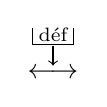
\begin{tikzpicture}[x=1em,y=1em,baseline=(rel.base)]
  \node[inner sep=0pt] (rel) at (0,0) {$\longleftrightarrow$};
  \node[inner sep=0pt] at (0,1.4) {\scriptsize déf};
  \draw (-.75,1.65)--(-.75,1.05)--(.75,1.05)--(.75,1.65);
  \draw[->] (0,1.02)--(0,.3);
\end{tikzpicture}}}}
\ \text{donnée de}\quad
\operatorname{Isom}_{\text{ens}}\left(
 \underset{\substack{\rotatebox{90}{$=$}\\(k^n-\unsure{(0)|(0}/k^*}}{\mathbb{P}^{n-1}(k)},P\right)
 /\operatorname{GP}(n-1,k)
\]

\figure{
\begin{tikzpicture}[x=\linewidth,y=1ex]
\draw (.29,1.5) -- (.58,1.5) .. controls (.61,1.5) and (.61,-.5) .. (.65,-.5) -- (.98,-.5);
\end{tikzpicture}}
\diagram{\begin{tikzcd}[ampersand replacement=\&,column sep=small,row sep=.6em]
\operatorname{Gl}(n,k)\arrow[r]\&\operatorname{Aff}(n,k)\arrow[r]\&\operatorname{GP}(n,k)\\
\substack{\text{vect. de dim $n$}\\\text{sur $k$}}\arrow[r,maps to,"\substack{\text{oubli}\\\text{origine}}"']
\&\substack{\text{espace affine de}\\\text{dim $n$ sur $k$}}
\arrow[r,maps to,"\substack{\text{espace proj.}\\\text{associé à}\\\text{l'esp. vect. \unsure{enveloppant|enveloppe}}}"']
\&\substack{\text{espace projectif}\\\text{de dim $n$ sur $k$}}
\end{tikzcd}}
% archive sheet number: 13
